% !TeX document-id = {fc3ccb1e-aeba-4c77-9990-74eef049f67c}
% !TeX TXS-program:compile = txs:///pdflatex/[--shell-escape]

\documentclass[glossy,aspectratio=169]{beamer}
\beamertemplatenavigationsymbolsempty
\usepackage[utf8]{inputenc}
\usepackage{DejaVuSans}
\renewcommand*\familydefault{\sfdefault}
\usepackage[fixed]{fontawesome5}

\useoutertheme{infolines}
\useinnertheme[realshadow,corners=2pt,padding=2pt]{chamfered}
\usecolortheme{whale}
\usepackage[ngerman]{babel}
\usepackage{graphics, graphicx}
\usepackage{color}
\usepackage{latexsym}
\usepackage{etoolbox}
\usepackage{subfig}
\usepackage{tikz}
\PassOptionsToPackage{hyphens}{url}
\usepackage{hyperref}
\usepackage{url}
\usepackage{qrcode}
\usepackage{eurosym}

% Override these to reproduce a build, if you run
% "nix-build --argstr date YYYY-MM-DD" you don't need to change them manually:
\year=\year
\month=\month
\day=\day

\newcommand{\semester}{SoSe 22}
\newcommand{\linkMaillists}{https://www.fsi.uni-tuebingen.de/infos/maillists/}
\newcommand{\linkErsti}{https://www.fsi.uni-tuebingen.de/du-bist-ersti/} % Maybe use this link
\newcommand{\linkAnmeldung}{https://eei.uni-tuebingen.de/}
\newcommand{\linkErstiheft}{https://teri.fsi.uni-tuebingen.de/anfiheft/}
\newcommand{\linkDiscord}{https://discord.gg/d4X2WjHWmQ}

\newcommand<>{\hover}[1]{\uncover#2{%
		\begin{tikzpicture}[remember picture,overlay]%
		\draw[fill,opacity=0.4] (current page.south west)
		rectangle (current page.north east);
		\node at (current page.center) {#1};
		\end{tikzpicture}}
}

\setbeamertemplate{headline}{}

\definecolor{pblue}{rgb}{0.13,0.13,1}
\definecolor{pgreen}{rgb}{0,0.5,0}
\definecolor{pred}{rgb}{0.9,0,0}
\definecolor{pgrey}{rgb}{0.46,0.45,0.48}
\definecolor{darkgreen}{rgb}{0,0.5,0}
\definecolor{fsiblue}{HTML}{000080}

\title{Fachschaftsvorstellung}
\author{\textbf{fsi}}

\begin{document}
    
%---------------------------------------------------------------------------
%   Title
%---------------------------------------------------------------------------
%\maketitle
\begin{frame}
    \centering
    \vspace{.5cm}
	
\includegraphics[width=0.8\textwidth]{pictures/fsilogo_neu.pdf}\\
	\vspace*{1cm}
	\begin{huge}
	   Hey! Wir helfen euch $\{\text{ins}\mid\text{im}\}$ Studium!
	\end{huge}

    \vspace{1.5cm}
    \semester
\end{frame}

%= = = = = = = = = = = = = = = = = = = = = = = = = = = = = = = = = = = = = = = =
%   Table of Contents
%   =================
%
%   1. Wer sind wir?
%   2. Was machen wir?
%   3. Mailinglisten
%   4. Wie lernt man Leute kennen
%       4.1 Ersti-Programm
%       4.2 Erstiheft
%       4.3 Discord
%   5. Mach doch mit!	
%= = = = = = = = = = = = = = = = = = = = = = = = = = = = = = = = = = = = = = = =


%-------------------------------------------------------------------------------
%   Wer sind wir?
%-------------------------------------------------------------------------------

\section{Wir, die FSI!}
\begin{frame}{\insertsection}
    \begin{figure}
        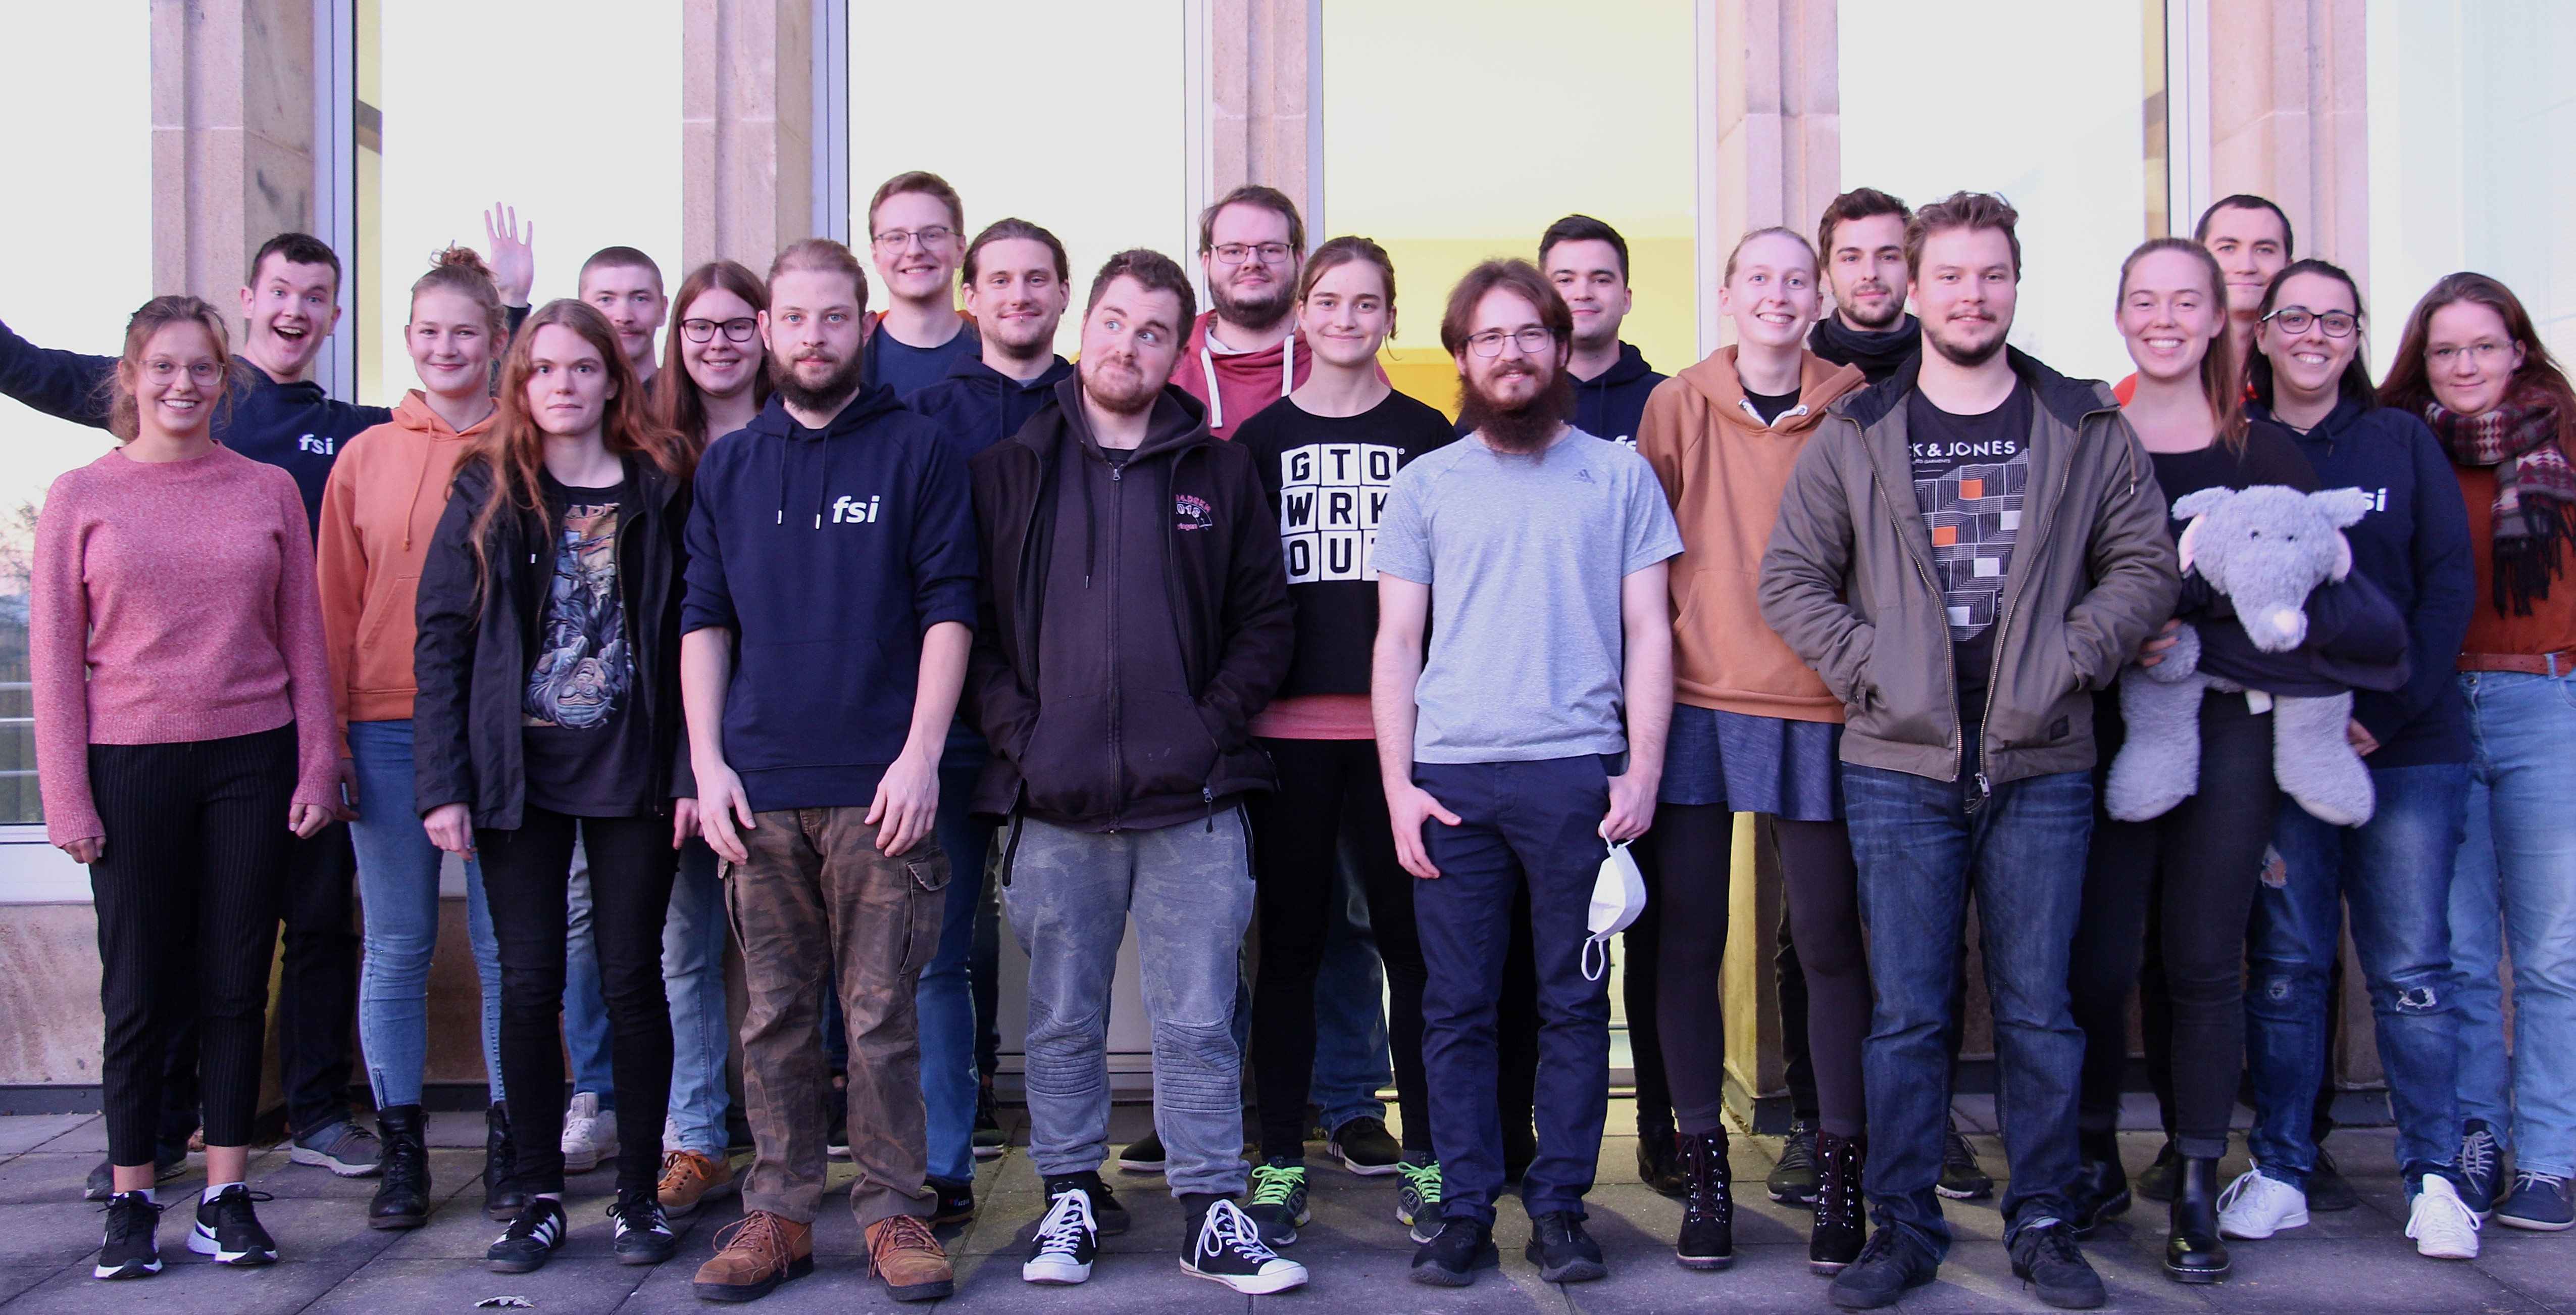
\includegraphics[height=.85\textheight]{pictures/fsi_22.jpg}
    \end{figure}

    \note{Hier labern wir sympathisch alá "Das da bin ich ohne Maske", 
          "Das ist der Tim", usw.}
\end{frame}



%-------------------------------------------------------------------------------
%   Was machen wir? Wir vertreten euch!
%-------------------------------------------------------------------------------

\section{Was machen wir?}
\begin{frame}{\insertsection}
    \begin{columns}
        \column{.5\textwidth}
        {\huge\itshape \textcolor{fsiblue}{Wir vertreten euch!}}
        
        \column{.5\textwidth}
        \begin{itemize}
            \item \textbf{Beratung/Betreung} bei deinen Problemen
            \item \textbf{Kontakt} zur Professorenschaft
            \item \textbf{Aktionen} und \textbf{Events}
                  \faMusic Clubhausfest (12.05.) und 
                  \faBeer Sommerfest (24.06.) 
            \item \textbf{Hochschulpolitik}: StuRa, FakRat
            \item \textbf{Gremien} wie Studienkommission, Prüfungsausschuss,
                  Berufungskommissionnen
        \end{itemize}
        
    \end{columns}
\end{frame}


%-------------------------------------------------------------------------------
%   Mailinglisten
%-------------------------------------------------------------------------------

\section{Mailinglisten}
\begin{frame}[t]{\insertsection}
    \textbf{Erstens:} Lest eure Uni-Mails!
    \footnote{also die wichtigen. Wie ihr Spam" wegfiltert haben wir für euch hier:
              \url{https://github.com/fsi-tue/workshops/blob/master/2019/05-8-unimails.pdf}}
    \begin{itemize}
        \item \textbf{info-studium}\\
              \textcolor{red}{\faExclamationTriangle 
                  Der einzige Weg des Fachbereich euch wichtige Informationen 
                  zukommen zu lassen. Anmeldung ist \textbf{PFLICHT}!
              \faExclamationTriangle}
        \item \textbf{info-talk}\\
              Für Informationen rund um Tübingen, der Informatik und dem Rest.
        \item \textbf{info-jobs}\\
              Jobangebote mit Bezahlung
    \end{itemize}
    \vfill
    \textbf{Anmeldung:} \url{\linkMaillists}
\end{frame}

\begin{frame}{Direkt anmelden!}
    \begin{columns}
        \column{.7\textwidth}
        \begin{enumerate}
            \item Auf die Seite gehen
            \item Im Textfeld oben eure \textbf{Email-Adresse} eintragen
            \item Den Button \textbf{\textsc{REGISTRIEREN}} anklicken
        \end{enumerate}
    
        \centering
        \vspace{1cm}
        {\huge\color{fsiblue} \faHandsWash Danke allerseits! }
                
        \column{.3\textwidth}
        \centering
        \qrcode[height=.9\linewidth]{\linkMaillists}
        \\[1em]
        \url{\linkMaillists}
    \end{columns}
\end{frame}


%-------------------------------------------------------------------------------
%   Wie lerne ich leute kennen?
%-------------------------------------------------------------------------------

\section{Wie lerne ich Leute kennen?}

%- - - - - - - - - - - - - - - - - - - - - - - - - - - - - - - - - - - - - - - -
\subsection{Ersti-Programm}

\begin{frame}{\insertsubsection}
    \begin{columns}
        \column{.7\textwidth}
        \begin{itemize}
            \large
            \item {\large\faDice} Spieleabend (12.04., 28.04.)
            \item {\large\faUtensils} Grillen (13.04.)
            \item {\large\faRoute} Stadtrallye (20.04.)
            \item {\large\faBeer} Kneipentour (20.04.)
            \item {\large\faHiking} Wanderung (24.04.)
        \end{itemize}
        \centering
        \vspace{1em}
        {\huge\color{fsiblue} Anmeldung \faLongArrowAltRight}
        
        \column{.3\textwidth}
        \centering
        \qrcode[height=.9\linewidth]{\linkAnmeldung}
        \\[1em]
        \url{\linkAnmeldung}
    \end{columns}
\end{frame}

\begin{frame}{Erstiheft}
    \begin{columns}
        \column{.7\textwidth}
        \begin{figure}
            \colorbox[gray]{.95}{
                
\includegraphics[height=.8\textheight]{pictures/erstiheft.pdf}}
        \end{figure}
        
        \column{.3\textwidth}
        \centering
        \qrcode[height=.9\linewidth]{\linkErstiheft}
        \\[1em]
        \url{\linkErstiheft}
    \end{columns}
\end{frame}

%- - - - - - - - - - - - - - - - - - - - - - - - - - - - - - - - - - - - - - - -
\subsection{Sonstiges}
\begin{frame}{Discord anyone?}
    \begin{columns}
        \column{.7\textwidth}
        \centering
        \textit{\Large Mit Leuten quatschen, Online-Spieleabende und 
                       Übungsblätter remote machen?}\\[1em]
        {\Huge\color{fsiblue}\faComments}
        
        
        \column{.3\textwidth}
        \centering
        \qrcode[height=.9\linewidth]{\linkDiscord}
        \\[1em]
        \url{\linkDiscord}
    \end{columns}
\end{frame}


%-------------------------------------------------------------------------------
%   Mach doch mit!
%-------------------------------------------------------------------------------

\section{Mach doch mit!}
\begin{frame}{\insertsection}
    \Large
    {\Huge\color{fsiblue} \faClock[regular]}   Donnerstags 18:30 Uhr \\[.5em]
    {\Huge\color{fsiblue} \faMapMarker*}       C125 - Sand 14 \\[.5em]
    \color{darkgray}
    {\Huge\color{fsiblue!50!darkgray} \faMapMarker*}       
                            \url{https://bbb.fsi.uni-tuebingen.de/b/luk-v3t-dvk}
\end{frame}

\end{document}
